
\chapter{Inequalities of coherent risk measures}
\label{chapter_inequalities}

Inequalities are the foundation of any analytical treatment of a subject. Here, we collect and prove many inequalities for coherent risk measures. Most of them are generalizations to inequalities that involve expectation.

We cannot find in the literature the inequalities that follow, so we believe these are new results. However, in \cite[Chapter 3]{zabarankinStatisticalDecisionProblems2016}, the authors presented similar probability inequalities for general risk measures.

\section{Elementary inequalities}\label{sec:elementary_inequalities}
\begin{prop}[Cauchy--Schwarz inequality]
For any sublinear, monotonic functional $\mathcal{F}$ on $\mathscr{L}^2$, and any $X, Y\in \mathscr{L}^2$, if $\mathcal{F}(XY) \le 0$, then 
\begin{equation}
\label{eq:csineq_crm}
\mathcal{F}(XY)^2 \le \mathcal{F}(X^2)\mathcal{F}(Y^2)
\end{equation}
Similarly, if $\mathcal{F}(-XY)\le 0$, then 
\begin{equation}
\label{eq:csineq_crm_2}
\mathcal{F}(-XY)^2 \le \mathcal{F}(X^2)\mathcal{F}(Y^2)
\end{equation}
\end{prop}
\begin{proof}
For the first case, let $\lambda =\mathcal{F}(XY)/\mathcal{F}(Y^2)$, and expand the right side of 
$$0\le \mathcal{F}((X-\lambda Y)^2)$$. 

The second case is converted to the first case by changing the sign of $X$.
\end{proof}

Jensen's inequality does not generalize easily. \cite[Theorem 3]{chenRiskMeasuresNonlinear2013} shows that any coherent risk measures that is a $g$-expectation obeys Jensen's inequality, but since we have no use for $g$-expectation in this thesis, this result will be skipped.

Two inequalities for expectations extend trivially via the dual representation of coherent risk measures (Proposition \ref{prop:dual_crm}).
\begin{prop}[H\"older inequality]
	For any closed, coherent risk measure $\mathcal{F}$ on $\mathscr{L}^2$, and any $p, q > 0$ such that $\frac 1 p + \frac 1 q = 1$, for any $X, Y\in \mathscr{L}^2$ with finite $\mathbb{E}(|X|^p), \mathbb{E}(|Y|^q)$, then 
	\begin{equation}
		\mathcal{F}(|XY|) \le \mathcal{F}(|X|^p)^{1/p} \mathcal{F}(|Y|^q)^{1/q}.
	\end{equation}
\end{prop}
\begin{proof}
	As in Equation \ref{eq:dual_crm}, take the dual representation of $\mathcal{F}$:
	$$\mathcal{F}(Z) = \sup_{\theta\in\Theta} \mathbb{E}_\theta(Z)$$
	Then
	\begin{align*}
		\mathcal{F}(|XY|) &= \sup_{\theta\in\Theta} \mathbb{E}_\theta(|XY|) \\
			&\le \sup_{\theta\in\Theta}\left( \mathbb{E}_\theta(|X|^p)^{1/p} \mathbb{E}_\theta(|Y|^q)^{1/q}\right) 
			\quad\text{ (H\"older inequality)}\\
			&\le \left(\sup_{\theta\in\Theta} \mathbb{E}_\theta(|X|^p)^{1/p}\right)
			\left(\sup_{\theta\in\Theta} \mathbb{E}_\theta(|Y|^q)^{1/q}\right)\\
			&= \left(\sup_{\theta\in\Theta} \mathbb{E}_\theta(|X|^p)\right)^{1/p}
			\left(\sup_{\theta\in\Theta} \mathbb{E}_\theta(|Y|^q)\right)^{1/q}\\
			&= \mathcal{F}(|X|^p)^{1/p}\mathcal{F}(|Y|^q)^{1/q}.
	\end{align*}
\end{proof}

\begin{prop}[Minkowski inequality]
	Under the same assumptions as above,
	\begin{equation}
	\mathcal{F}(|XY|) \le \mathcal{F}(|X|^p)^{1/p} + \mathcal{F}(|Y|^q)^{1/q}.
	\end{equation}
\end{prop}
\begin{proof}
	Essentially the same as the previous proof.
\end{proof}

\section{Concentration inequalities}\label{sec:tail_ineq}
A "nice" random variable should be "far" to its expectation with a small probability, that is, its value should be concentrated around its expectation. Concentration inequalities quantify this vague statement in various ways.

In this section, we prove generalizations of Markov, Chebyshev, Chernoff, Hoeffding, Bennett, and Bernstein's inequalities. These inequalities are the most important tail inequalities, heavily used in all parts of statistics, probability, and machine learning. As one example, the Hoeffding inequality is the basis of the popular Monte Carlo tree search algorithm UCT\cite{kocsisBanditBasedMonteCarlo2006}.

\begin{prop}[Markov's inequality]\label{prop:markov}
Given any monotonically increasing $\phi : [0, \infty) \to [0, \infty)$, any $a \ge 0, X\in\mathscr{L}$, and monotonic, positively homogenous functional $\mathcal{F}$,
\begin{equation}
\label{eq:markov}
\mathcal{F}(\phi(|X|)) \ge \phi(a) \mathcal{F}(1_{|X|\ge a})
\end{equation}

Similarly, if $\phi: \mathbb{R} \to [0, \infty)$ is monotonically increasing, then for any $a$, 
\begin{equation}
\label{eq:markov_2}
\mathcal{F}(\phi(X)) \ge \phi(a) \mathcal{F}(1_{X\ge a})
\end{equation} 
\end{prop}
\begin{proof}
For the first case, since $\phi(|X|) \ge \phi(a) 1_{|X|\ge a}$, by monotonicity of $\phi$ and positive homogeneity of $\mathcal{F}$, 
$$\mathcal{F}(\phi(|X|)) \ge  \mathcal{F}(\phi(a)1_{|X|\ge a}) = \phi(a)\mathcal{F}(1_{|X|\ge a}). $$

Similarly for the second case.
\end{proof}

\begin{prop}[Chebyshev's inequality]
Given any $a > 0, X\in\mathscr{L}$, and monotonic, positively homogenous functional $\mathcal{F}$,
\begin{equation}
\label{eq:chebyshev}
\mathcal{F}(1_{|X|\ge a})\le \frac{1}{a^2}\mathcal{F}(X^2) 
\end{equation}
\end{prop}
\begin{proof}
Let $\phi(a) = a^2$ in the first Markov's inequality.
\end{proof}

\begin{prop}[Chernoff bound]
Given any $t > 0, X\in\mathscr{L}$, and monotonic, positively homogenous functional $\mathcal{F}$,
\begin{equation}
\label{eq:chernoff}
\ln\mathcal{F}(1_{X\ge t}) \le -\sup_{a \ge 0}(ta - \ln\mathcal{F}(e^{aX}))
\end{equation}
\end{prop}
\begin{proof}
Let $\phi(x) = e^{tx}$ in the second Markov's inequality, to get 
$$\mathcal{F}(1_{X\ge t}) \le e^{-ta}\mathcal{F}(e^{tX})\quad \text{for any } a > 0.$$

Then take logarithm on both sides, and take the infimum over $a > 0$ on the right side. 

Note that the $a = 0$ case gives $\ln\mathcal{F}(1_{X\ge t}) \le 0$, which is trivially true, since 
$$\mathcal{F}(1_{X\ge t}) \le \mathcal{F}(1) = 1,$$
so it can be incorporated safely into the infimum.
\end{proof}

We record a particularly useful case for \cvar:

\begin{cor}[Chernoff bound for \cvar]
	\label{thm:chernoff_cvar}
	Given any real random variable $X$ with finite first moment, any $\alpha \in [0, 1]$, and any $a > \var_\alpha(X)$, we have 
	\begin{equation}
	\label{eq:chernoff_cvar}
		Pr(X \ge a) \le {\overbar{\alpha}} \inf_{t > 0} \cvar_\alpha(e^{tX}) e^{-ta}
	\end{equation}
\end{cor}
\begin{proof}
	In Chebyshev's inequality, replace $\mathcal{F}, a, X$ by $\cvar_\alpha, 1, e^{t(X - a)/2}$, to obtain
	$$\cvar_\alpha(1_{X \ge a}) = \cvar_\alpha(1_{e^{t(X-a)/2} \ge 1}) \le \cvar_\alpha(e^{t(X-a)}) = \cvar_\alpha(e^{tX}) e^{-ta}$$
	for any $ t> 0$.
	
	Since $a > \var_\alpha(X)$, we have $Pr(X \ge a) \le {\overbar{\alpha}}$, and so
	$$\cvar_\alpha(1_{X \ge a}) = \min(1, Pr(X \ge a)/{\overbar{\alpha}}) = Pr(X \ge a)/{\overbar{\alpha}}.$$
	Optimize over $t$ to obtain the result.
\end{proof}

\begin{prop}[Hoeffding's lemma]
For any coherent risk measure $\mathcal{F}$ on $\mathscr{L}$, and $X$ such that $Pr(a\le X \le b) = 1$, let 
$$c(t) = \frac{\mathcal{F}(X) + \mathcal{F}(-X)}{e^{t(b-a)} - 1},$$
then for any $t\in\mathbb{R}, t\neq 0$,
\begin{equation}
\label{eq:hoeffding_lemma}
\mathcal{F}(\exp{[t(X - \mathcal{F}(X) - c(t))]}) \le \exp\left(\frac 1 8 (b-a)^2 t^2\right)
\end{equation}
\end{prop}
\begin{proof}
Rewrite $X$ as a convex sum of $a, b$:
$$X = \theta b + (1-\theta) a.$$
By convexity of $x\mapsto e^{tx}$, 
$$e^{tX} \le \theta e^{tb} + (1-\theta)e^{ta} = \frac{1}{b-a}((X-a)e^{tb} + (b-X)e^{ta})$$
Then by the coherence of $\mathcal{F}$, 
$$\mathcal{F}(e^{tX}) \le \frac{e^{tb}}{b-a}(\mathcal{F}(X) -a ) + \frac{e^{ta}}{b-a}(\mathcal{F}(-X) + b)$$

Replace $X$ by $X - \mathcal{F}(X) - c(t)$ in the above equation, and simplify, using translation invariance of $\mathcal{F}$, to cancel out the $\mathcal{F}$ terms on the right. This yields
\begin{align*}
\mathcal{F}(\exp{[t(X - \mathcal{F}(X) - c(t))]}) &\le \frac{be^{ta}-a e^{tb}}{b-a} = e^{g(u)}
\end{align*}
where 
$$
\begin{cases}
u = t(b-a)\\
g(u) = -\gamma u + \ln(1-\gamma + e^u \gamma)\\
\gamma = -\frac{a}{b-a}
\end{cases}
$$
Since $$
\begin{cases}
g(0) = 0\\
g'(0) = 0\\
g''(u) \le \frac 1 4 \quad \text{for } u\ge 0
\end{cases}
$$
we have
$$g(u) \le \frac 1 8 u^2 = \frac 1 8 t^2(b-a)^2$$
yielding the result.
\end{proof}

Hoeffding's lemma is often used to prove Hoeffding's inequality. However, the proof does not generalize immediately to general CRM, or even \cvar, because it depends on that for any two independent $X, Y\in \LL^1$, $\E(XY) \le \E(X)\E(Y)$, which is false for $\cvar$ in general:

\begin{ex}
	Given independent $X, Y$, it is not the case that $\mathcal{F}(XY) = \mathcal{F}(X) \mathcal{F}(Y)$. In fact, even for $\cvar_\alpha$, it is possible for one side to be arbitrarily greater than the other.
	
	Let $X, Y$ both have the distribution on $\{-T, T\}$ defined by 
	$$Pr(X = -T) = \frac 3 4, \quad Pr(X = T) = \frac 1 4$$ 
	$T$ being a positive constant, then 
	$$\cvar_{1/2}(X) = \cvar_{1/2}(Y) = 0 $$
	$$\cvar_{1/2}(XY) = T^2$$
	so $\cvar_{1/2}(XY)$ can be arbitrarily greater than $\cvar_{1/2}(X)\cvar_{1/2}(Y)$.
\end{ex}

However, when $X, Y\ge 0$ almost surely, we do have:
\begin{prop}
	For any two independent $X, Y\in \LL^1$ that are almost surely non-negative, and any $\alpha \in [0, 1]$, 
	\begin{equation}
		\cvar_\alpha(XY) \le \cvar_\alpha(X)\cvar_\alpha(Y).
	\end{equation}
\end{prop}
\begin{proof}	
	By continuity of $\cvar_\alpha$ with respect to $\alpha$, it suffices to prove this for all rational $\alpha \in(0, 1)$. 
	
	By closedness of $\cvar_\alpha$, it suffices to prove this for all $X, Y$ in a dense subset of $\LL^1$.
	
	For any $\alpha = \frac m n$, with $0< m < n$ integers, we prove this proposition for the dense subset of $\LL^1$:
	$$ \left\{X\in \LL^1 : X \text{ has distribution } \frac 1{N} \sum_{i= 1}^{N} \delta_{x_i}, n\text{ divides }N, \text{ and all } x_i \ge 0 \right\}.$$
	This subset is chosen, because it makes $\cvar_\alpha(X)$ easy to calculate: 
	$$\cvar_\alpha(X) = \frac 1{{\overbar{\alpha}} N}\sum\left(\text{the biggest } {\overbar{\alpha}} N \text{ terms of }x_i\right)$$
	for any such $X$. That is, the average of the largest ${\overbar{\alpha}} N$ terms of the sequence. We write this as $\overbar x_{{\overbar{\alpha}} N}$
	
	Now, it remains to show that for any two such sequences $(x_i)_{i=1}^N,  (y_i)_{i=1}^N$, we have 
	$$\overbar{(xy)}_{\alpha N^2} \le \overbar x_{{\overbar{\alpha}} N} \overbar y_{{\overbar{\alpha}} N}$$ 
	
	The proof proceeds by modifying the sequences $X, Y$ until they become trivial, preserving the inequality along the way.
	
	Let $0\le y_1 \le \cdots \le y_N$, so that 
	$$\overbar y_{{\overbar{\alpha}} N} = \frac 1{{\overbar{\alpha}} N}\sum_{i=\alpha N + 1}^{N}y_i.$$
	Now let $\epsilon = y_N - y_{\alpha N + 1}$, and decrease $y_N$ by $\epsilon$. This decreases $\cvar_\alpha(X)\cvar_\alpha(Y)$ by $\frac{\epsilon}{{\overbar{\alpha}} N} \cvar_\alpha(X)$.
	
	Since it decreases the entries in the list $\{x_iy_j\}_{i, j \in[N]}$ by $\epsilon x_1, ..., \epsilon x_N, 0, 0, ... 0$, it decreases $ \cvar_\alpha(XY)$ by at most 
	$$\frac{\epsilon}{{\overbar{\alpha}} N^2} (x_1 + \cdots + x_N) \le \frac{\epsilon}{{\overbar{\alpha}} N} \cvar_\alpha(X).$$
	Thus, each such reduction decreases $\cvar_\alpha(X)\cvar_\alpha(Y)$ more than $\cvar_\alpha(XY)$. So if after such decrease, the inequality holds, the inequality still holds before the decrease.
	
	After doing this decrease for ${\overbar{\alpha}} N$ times on $y$, then on $X$, we have the largest ${\overbar{\alpha}} N$ entries of $x$ equal, and the same for $Y$, and so 
	$$\cvar_\alpha(X)\cvar_\alpha(Y) = \max(X)\max(Y) = \max(XY) \ge \cvar_\alpha(XY).$$
 \end{proof}

Now we are ready to prove generalized Hoeffding, Bennett, and Bernstein's inequalities.

\begin{defn}
	The \textbf{cumulant generating function} of $\cvar_\alpha$ is 
	\begin{equation}
		K_{\alpha X}(t) = \log{\Ca(e^{tX})}.
	\end{equation}
\end{defn}

\begin{prop}[Hoeffding's inequality]\label{prop:hoeffding}
Let $X_1, ... X_n$ be a sequence of independent real random variables, with each $X_i \in [a_i, b_i]$ almost surely. Let $\alpha \in [0, 1)$, then $\forall t > 0$, 

\begin{equation}
\begin{aligned}
	Pr &\left(\sumn (X_i - \Ca(X_i)) \ge t\right) \le \\ &{\overbar{\alpha}} \exp\left(-\frac{2t^2}{\sumn (b_1 - a_i)^2} + \sumn \frac{\Ca(X_i) + \Ca(-X_i)}{b_i - a_i}\right).
\end{aligned}
\end{equation}
\end{prop}
\begin{proof}
	Define for all $i\in[n]$,
	$$ c_i(s) = \frac{\Ca(X_i) + \Ca(-X_i)}{e^{s(b_i - a_i)} - 1}$$
	
	For any $t$, and any $s > 0$, such that $t + \sumn (\Ca(X_i) + c_i(s)) > \var_\alpha(\sumn X_i)$, we have by Chernoff bound,
	\begin{align*}
		\frac 1 {\overbar{\alpha}} Pr\Bigg( \sumn X_i \ge t &+\left. \sumn (\Ca(X_i) + c_i(s))\right) \\
		&\le \Ca(e^{s\sumn X_i}) e^{-st - s\sumn (\Ca(X_i) + c_i(s))} \\
		&= \Ca\left(\prod_{i=1}^n e^{s(X_i - \Ca(X_i) -c_i(s))}\right)e^{-st}\\
		&\le e^{-st} \prod_{i=1}^n \Ca\left( e^{s(X_i - \Ca(X_i) -c_i(s))}\right)\\
		&\le \exp\left(-st + \frac{s^2}{8}\sumn(b_i- a_i)^2\right)
	\end{align*}
	So for any $t > \var_\alpha(\sumn X_i)$, and any $s > 0$, 
	$$
	\frac 1 {\overbar{\alpha}} Pr\left(\sumn X_i \ge t\right) 
	\le \exp\left(-st + s\sumn\Ca(X_i) + s\sumn c_i(s) + \frac 18 s^2 \sumn(b_i - a_i)^2\right)
	$$
	Since for all $s>0$, 
	$$sc_i(s) \le \frac{\Ca(X_i) + \Ca(-X_i)}{b_i - a_i}$$
	we have
	$$ \begin{aligned}
	\frac 1 {\overbar{\alpha}} Pr\left(\sumn X_i \ge t\right) 
	\le \exp&\left(-st + s\sumn\Ca(X_i) + \frac 18 s^2 \sumn(b_i - a_i)^2 + \right.\\
	& \left. \sumn \frac{\Ca(X_i) + \Ca(-X_i)}{b_i - a_i}\right).
	\end{aligned}
	$$
	So for all $t > \var_\alpha(\sumn X_i)$, 
	$$ \begin{aligned}
 	Pr\left(\sumn X_i \ge t\right) 
	\le {\overbar{\alpha}} \inf_{s > 0}\exp&\left(-st + s\sumn\Ca(X_i) + \frac 18 s^2 \sumn(b_i - a_i)^2 + \right.\\
	& \left. \sumn \frac{\Ca(X_i) + \Ca(-X_i)}{b_i - a_i}\right).
	\end{aligned}
	$$
	When $ t \le \sumn\Ca(X_i)$, the right side is $\ge {\overbar{\alpha}}$, which makes the inequality useless, as the left side is $\le {\overbar{\alpha}}$ from $t > \var_\alpha(\sumn X_i)$. 
	
	So assume that $ t > \sumn \Ca(X_i)$, which implies $ t> \var_\alpha(\sumn X_i)$. Then, taking the minimum on the right side gives 
	$$
	\begin{aligned}
	Pr &\left(\sumn X_i \ge t\right) \le \\ &{\overbar{\alpha}} \exp\left(-\frac{2\left(t - \sumn \Ca(X_i)\right)^2}{\sumn(b_i - a_i)^2} + \sumn\frac{\Ca(X_i) + \Ca(-X_i)}{b_i - a_i}\right)
	\end{aligned}
	$$
	which is equivalent to what we need to prove.
\end{proof}


\begin{prop}[Bennett's inequality]
	Let $X_1, ... X_n$ be a sequence of independent real random variables, with each $\Ca(X_i)  = 0$, and $X_i \le a$ almost surely. Let $\alpha \in [0, 1)$, and let 
	$$v_\alpha = \sumn\Ca(X_i^2),$$
	then $\forall t > 0$, 
	
	\begin{equation}
	\begin{aligned}
	Pr\left(\sumn X_i \ge t\right) \le {\overbar{\alpha}} \exp\left(-\frac{v_\alpha}{a^2}h\left(\frac{at}{v_\alpha}\right)\right)
	\end{aligned}
	\end{equation}
	where 
	\begin{equation}
	h(t) = (1 - t)\ln(1+t) - t
	\end{equation}
\end{prop}
\begin{proof}
	Let 
	$$\psi(x) = e^x - 1 - x$$
	so that 
	$$
	\psi(x) = 
	\begin{cases}
		\le \frac 1 2 x^2\quad \text{ when } x\le 0 \\
		\ge \frac 1 2 x^2\quad \text{ when } x\ge 0
	\end{cases}
	$$
	As in the previous proof, for all $ s > 0$, $t > \var_\alpha(\sumn X_i)$, 
	$$
	\frac 1{\overbar{\alpha}} Pr\left(\sumn X_i \ge t\right) \le e^{-st}\prod_{i=1}^n \Ca\left(e^{sX_i}\right)
	$$
	Then 
	$$ 
	\begin{aligned}
		\Ca\left(e^{sX_i}\right) &= 
			\Ca\left(1 + sX_i + \psi(sX_i)\right) \\
		&\le 1 + s\Ca(X_i) + \Ca(\psi(sX_i)) \\
		&= 1 + \Ca(\psi(sX_i))\\
		&\le \exp\left( \Ca(\psi(sX_i)) \right)
	\end{aligned}
	$$
	So, 
	$$
	 Pr\left(\sumn X_i \ge t\right) \le {\overbar{\alpha}} \exp\left(-st + \sumn \Ca(\psi(sX_i)) \right)
	$$
	Let $X_i^+ = \max(X_i, 0), X_i^- = \max(-X_i, 0)$, so that $X_i = X_i^+ - X_i^-$, and by convexity of $\psi$, 
	$$
	\psi(sX_i) \le \psi(sX_i^+) + \psi(-sX_i^-)
	$$
	By bounds on $\psi$, 
	$$\psi(-sX_i^-) \le \frac 12 s^2 (X_i^-)^2 \le  \frac{(X_i^-)^2}{a^2}\psi(as) $$
	For any $s > 0, x\in[0, 1]$, 
	$$\psi(sx) = \frac 12 s^2x^2 + \frac 16 s^3 x^3 + \cdots \le x^2 (\frac 12 s^2 + \frac 16 s^3 + \cdots) = x^2 \psi(s) $$
	So 
	$$\psi(sX_i^+) = \psi(as(X_i/a)^+) \le \frac{(X_i^+)^2}{a^2}\psi(as) 
	$$
	So 
	$$\psi(sX_i) \le \psi(as) \frac{1}{a^2} \left((X_i^+)^2 + (X_i^-)^2\right) = \frac{\psi(as)}{a^2}X_i^2$$
	By monotonicity and positive homogeneity of $\Ca$,
	$$\Ca(\psi(sX_i)) \le \frac{\psi(as)}{a^2}\Ca(X_i^2)$$
	so
	$$
	Pr\left(\sumn X_i \ge t\right) \le {\overbar{\alpha}} \exp\left(-st + \frac{v_\alpha \psi(as)}{a^2}\right)
	$$
	for any $s > 0$. Optimizing the right side by $s = \frac 1a \ln(1 + at/v_\alpha)$, we get the desired inequality.
\end{proof}

Using the simple inequality
$$\forall t\ge 0, \quad h(t) \ge \frac{t^2}{2 + 2t/3} $$
we obtain
\begin{cor}[Bernstein's inequality]
	Let $X_1, ... X_n$ be a sequence of independent real random variables, with each $\Ca(X_i)  = 0$, and $X_i \le a$ almost surely. Let $\alpha \in [0, 1)$, and let 
	$$v_\alpha = \sumn\Ca(X_i^2),$$
	then $\forall t > 0$, 
	
	\begin{equation}
	\begin{aligned}
	Pr\left(\sumn X_i \ge t\right) \le {\overbar{\alpha}} \exp\left(-\frac{t^2}{2v_\alpha + 2at/3}\right)
	\end{aligned}
	\end{equation}
\end{cor}

\subsection{A conjecture}
The conditional \cvar can be defined in the same way as conditional expectation. So for example, if $X, Y\in\mathscr{L}^1$ are independent, then $\Ca(X|Y) = \Ca(X)$.

The Law of Total Expectation states that 
\begin{equation}
\E(X) = \E(\E(X|Y))
\end{equation}
The following conjecture was numerically found and verified for several million examples of discrete $X, Y$:
\begin{conj}[Law of total \cvar]\label{conj:total_cvar}
	For any two independent $X, Y\in \LL^1$ that are almost surely non-negative, and any $\alpha \in [0, 1)$, 
	\begin{equation}
	\Ca(X) \le \frac{1}{\overbar\alpha}\Ca(\Ca(X|Y)).
	\end{equation}
	Further, this is sharp in that for any $\epsilon\in(0, 1)$, $\frac{1}{\overbar\alpha}$ cannot be replaced by $\frac{1}{\overbar\alpha^{1-\epsilon}}$
\end{conj}

In proofs of martingale inequalities of expectation, such as McDiarmid's inequality and Doob's martingale inequality, the law of total expectation is used, so it stood to reason that a law of total \cvar would be required for a proof of martingale inequalities for \cvar. 

Unfortunately, even assuming the conjecture to be true, no valuable generalization of martingale inequalities to \cvar were discovered.

\section{Statistical learning theory (SLT)}
Learning theory is the theoretical counterpart of practical machine learning, and one of its main branches is statistical learning theory (SLT). For a historical overview up to 1999, see \cite[Introduction]{vapnikNatureStatisticalLearning2000}. For a detailed introduction to SLT, see \cite{bousquetIntroductionStatisticalLearning2003}.

SLT models the problem of learning by positing a \textbf{learner} who is trying to find the best \textbf{model} out of a \textbf{class of models}, given some \textbf{training data}.

\subsection{Overview of SLT}
Formally, let $\mathcal{X}$ be a nonempty set called \textbf{feature space}, and $\mathcal{Y}$ be another nonempty set called \textbf{label space}. Let there be a probability distribution $\mu$ on $\mathcal{Z} = \mathcal{X}\times\mathcal{Y}$. This specifies the learning problem.

For example, suppose the problem is to predict the height based on biological sex only, the feature space would be $\{\text{male}, \text{female}\}$, and the sample space $[0, \infty)$. The distribution $\mu$ is the probability distribution of a random person from the population having the specified sex and height. In particular, $\mu(\text{male}, [150, 160])$ is the probability that a random person would be male and having height between $150$ and $160$ cm.

The learner is given a sequence of $n$ \textbf{training data} sampled from $\mu$, that is, it is given 
$$Z^n = (Z_1, \cdots, Z_n) \in \mathcal{Z}^n$$

The learner already knows $\mathcal{X}, \mathcal{Y}$, so it can start with the \textbf{hypothesis class} $\mathcal{H}$, a set of \textbf{hypotheses} $h: \mathcal{X}\to \mathcal{Y}$. 

The problem of the learner, then, is to find the best $h_{Z^n}$, given training data $Z^n$.

To formalize "best", a \textbf{loss function} $\ell: \mathcal{Y} \times \mathcal{Y} \to [0, \infty)$ is defined, such that $\ell(y, y')$ measures how different $y, y'$ are. Given a hypothesis $h$, and a new data point $(x, y)$, $\ell(h(x), y)$ measures how badly the hypothesis errs on the data point. 

The simplest loss function is:
\begin{defn}[0-1 loss]
The \textbf{0-1 loss} is 
\begin{equation}
\ell_{01}(y, y') = \begin{cases}
1 \quad \text{if } y \neq y',\\
0 \quad \text{else.}
\end{cases}
\end{equation}
\end{defn}
More complex loss functions are often used, such as the quadratic loss, widely used in problems where the label space is continuous rather than discrete:
\begin{equation}
\ell_{01}(y, y') = (y-y')^2
\end{equation}
however, we have not generalized our results to such loss functions.

To judge the overall performance of hypothesis $h$, the expectation of loss is used:
\begin{defn}[Expected loss function]
\begin{equation}
\loss(h, \mu) = \mathbb{E}_{(X, Y)\sim \mu}(\ell(h(X), Y))
\end{equation}

where the subscript of $\mathbb{E}_{(X, Y)\sim \mu}$ means that $(X, Y)$ are random variables with joint probability measure $\mu_{(X, Y)} = \mu$.
\end{defn}

Suppose the learner knows $\mu$, then it could just return the optimal solution (sometimes called the \textbf{Bayes classifier})
$$h^* = \argmin_{h\in \mathcal{H}} \loss(h, \mu), $$
with minimal loss (the \textbf{Bayes risk})
$$L^* = \min_{h\in \mathcal{H}} \loss(h, \mu) = \loss(h^*, \mu).$$
But almost always, $\mu$ is inaccessible, and the learner may only access $Z^n$, with which it constructs an approximation of $\mu$, with which it selects a good hypothesis $h_{Z^n}$, such that $(\loss(h_{Z^n}, \mu) - L^*)$ is small. 

However, if $Z^n$ happens to be a very unlucky draw, it would give a bad approximation of $\mu$, from which the learner has no chance of learning well. To deal with such unlucky cases, instead of perfectly reliable learning, the concept of probably approximately correct (PAC) learning
\footnote{As a historical note, PAC-learning is proposed by Leslie Valiant in 1984 \cite{valiantTheoryLearnable1984}, and Valiant is quite enamored with it, recently proposing that the concept of evolvability, a fundamental notion of biological evolution and a significant ingredient in the explanation of life on earth, is a special case of PAC-learnability \cite{valiantEvolvability2009}.}
 is used:

\begin{defn}[PAC-learnability]
\label{defn:pac}
Given a hypothesis class $\mathcal{H}$ on the spaces $\mathcal{X}, \mathcal{Y}$, the hypothesis class is \textbf{PAC-learnable} if there exists a \textbf{learner function} $Z^n \mapsto h_{Z^n}$, such that for any probability measure $\mu$ over $\mathcal{X}\times \mathcal{Y}$, and any $\epsilon > 0, \delta > 0$, there exists some $N\in \mathbb{N}$, such that for any integer $n > N$, 

\begin{equation}
\label{eq:pac}
Pr_{(X, Y)\sim \mu}(\loss(h_{Z^n}, \mu) - L^* < \epsilon) > 1- \delta
\end{equation}
where $L^* = \min_{h\in \mathcal{H}} \loss(h, \mu)$.
\end{defn}

In other words, given enough samples, the probability of learning a bad hypothesis is low, regardless of the truth $\mu$. This can be reformulated as a convergence in probability: 
\begin{equation}
\min_{h\in \mathcal{H}} \loss(h, \mu_{Z^n})\probconv  \min_{h\in \mathcal{H}} \loss(h, \mu)
\end{equation}

In other words, 
$$\min_{h\in \mathcal{H}} \loss(h, \mu_{Z^n}) $$ 
is a \textbf{consistent estimator} of $\min_{h\in \mathcal{H}} \loss(h, \mu) $.

Just from the definition, it is unclear whether any nontrivial learning problem is PAC-learnable. However, as it turns out, even the most naive learner, the empirical risk minimizer (ERM), can PAC-learn some nontrivial problems, as will be demonstrated in Theorem \ref{theorem:funtheo_slt}.

\begin{defn}[Empirical risk minimizer]\label{defn:erm}
Given a loss function $\ell$ and a hypothesis class $\mathcal{H}$, its associated empirical risk minimizer is defined by 
\begin{equation}
\label{eq:erm}
h_{Z^n} = \argmin_{h\in\mathcal{H}} \frac 1 n \sum_{i = 1}^n \ell(h(x_i), y_i)
\end{equation}
where $Z^n = ((x_1, y_1), ..., (x_n, y_n))$. It is often written as $ERM_{\mathcal{H}}$, with $\ell$ elided.
\end{defn}

In other words, upon receiving the training samples $Z^n$, it constructs $\mu_{Z^n}$ as the empirical approximation of $\mu$, then chooses the hypothesis $h\in\mathcal{H}$ that minimizes $\loss(h, \mu_{Z^n})$, 

\begin{notn}
For any $Z^n\in \mathcal{Z}^n$, $\mu_{Z^n}$ is the empirical distribution on $\mathcal{X}\times\mathcal{Y}$ defined by
\begin{equation}
	\mu_{Z^n} = \frac 1 n \sum_{i=1}^n \delta_{(X_i, Y_i)}
\end{equation}
\end{notn}

So we can more succinctly write Equation \ref{eq:erm} as 
\begin{equation}
\label{eq:erm_2}
h_{Z^n} = \argmin_{h\in\mathcal{H}} \loss(h, \mu_{Z^n})
\end{equation}



For an ERM learner to perform well, it must receive a training sample $Z^n$ that closely represents $\mu$. This can be formalized by the concept of 
\begin{defn}[$\epsilon$-representative sample]
A sample $Z^n$ is \textbf{$\epsilon$-representative sample} with respect to $\mathcal{H}$ if 
\begin{equation}
\sup_{h\in\mathcal{H}}| \loss(h, \mu_{Z^n}) - \loss(h, \mu)|\le \epsilon
\end{equation}
\end{defn}

Certain hypothesis classes can be easily $\epsilon$-represented, while others cannot. For example, with respect to the trivial class $\mathcal{H} = \{h\}$ with only one hypothesis allows any $Z^n$ to well, \textit{trivially} $0$-represent $\mu$. In contrast, if $\mathcal{H}$ is big, it will be difficult to represent $\mu$ well, since there is likely a $h\in \mathcal{H}$ that fits $Z^n$ very well, but fits $\mu$ poorly. This is essentially one manifestation of the \textbf{problem of overfitting}.

To formalize this notion of certain hypothesis classes being easier to allow good representation, we define:

\begin{defn}[Uniform convergence]
A hypothesis class $\mathcal{H}$ has uniform convergence property if there exists $n_{\mathcal{H}}: (0, 1)\times(0, 1) \to \mathbb{N}$, such that for any distribution $\mu$ over $\mathcal{X}\times\mathcal{Y}$, for any $\epsilon, \delta \in (0, 1)$, and any $n > n_{\mathcal{H}}(\epsilon, \delta)$, we have 
\begin{equation}
  Pr_{Z^n\sim \mu^n}(Z^n \text{ is }\epsilon\text{-representative}) > 1 - \delta
\end{equation}
\end{defn}
To say that $\mathcal{H}$ has uniform convergence is to say that a uniform weak law of large numbers holds. In detail,  for any hypothesis $h\in \mathcal{H}$ and any probability distribution $\mu$ over $\mathcal{X}\times \mathcal{Y}$, let $(z_n)_n$ be an IID sequence sampled from $\mu$, then 
$$\loss(h, \mu_{Z^n} ) = \frac 1 n \sum_{i = 1}^n \ell(h(x_i), y_i)\probconv \loss(h, \mu)$$
and this convergence in probability is uniform over $\mu$ and $h$.

That $\mathcal{H}$ is uniformly convergent is a strictly stronger hypothesis than that $ERM_\mathcal{H}$ is a  PAC-learner. To see this, note that the ERM learner is a PAC-learner if
$$\min_{h\in \mathcal{H}} \loss(h, \mu_{Z^n} ) \probconv \min_{h\in \mathcal{H}} \loss(h, \mu)$$
uniformly over $\mu$. This has one less uniformity condition, and thus weaker.

\begin{prop}
\label{prop:uniconv}
If a hypothesis class is uniformly convergent, then the $ERM_\mathcal{H}$ learner is a PAC-learner.
\end{prop}
\begin{proof}
Given any distribution $\mu$, let the Bayes hypothesis be $h^*$ and the Bayes loss be $L^*$. Now, for any $\epsilon, \delta \in (0, 1)$, and any $n > n_{\mathcal{H}}(\epsilon, \delta)$, let $Z^n$ be the training data sampled out of $\mu^n$, and $h_{Z^n}$ be the hypothesis produced by the $ERM_{\mathcal{H}}$ learner.

With probability above $1- \delta$, $Z^n$ is $\epsilon$-representative, then we have 
\begin{align*}
\loss(\mu, h_{Z^n}) &\le \loss(\mu_{Z^n}, h_{Z^n}) + \epsilon 
&\le \loss(\mu_{Z^n}, h^*) + \epsilon  
&\le \loss(\mu, h^*) + 2\epsilon 
&= L^* + 2\epsilon
\end{align*}

Thus 
$$|\loss(\mu, h_{Z^n}) - L^*| \le  2\epsilon.$$

Thus
$$Pr_{Z^n\sim \mu^n}(|\loss(\mu, h_{Z^n}) - L^*| \le  2\epsilon) \ge 1-\delta.$$
\end{proof}

In general, any learner must balance between too much overlearning and underlearning. Underlearning occurs when the learner fails to extract sufficient information from its training data, while overlearning occurs when the learner extracts too much from its training data.

Consider a human pupil learning from a textbook on arithmetics. An underlearner might read through the textbook and remain the same as before, while an overlearner might memorize every single word, but fail to do any problem that does not appear in the book.

For the $ERM_{\mathcal{H}}$ learner, its hypothesis class $\mathcal{H}$ is the deciding factor for whether it  would underlearn or overlearn. Intuitively, if $\mathcal{H}$ is small, for example, having only size 2, then no matter how rich the training samples are, the learner could only encode one bit of information in its final choice of hypothesis. One might say that the learner has only one bit of memory. This is a severe underlearner. If $\mathcal{H}$ is too big, for example, containing every single function of type $\mathcal{X}\to\mathcal{Y}$, then the $ERM_{\mathcal{H}}$ learner would simply "memorize" the whole training sample, with no regard for generalization outside it. Figure \ref{fig:over_and_underlearning} depicts these two pathologies of learning.

\begin{figure}
	\centering
	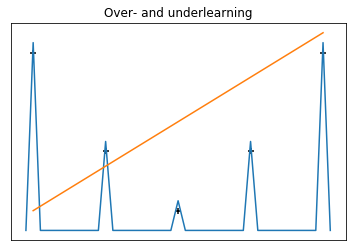
\includegraphics[width=0.6\linewidth]{over_and_underlearning}
	\caption{Illustration of over- and underlearning. The black crosses are the training samples. The straight line is the hypothesis learned by an underlearner, while the spiky line is the hypothesis learned by an overlearner.}
	\label{fig:over_and_underlearning}
\end{figure}

The key to a good $ERM_{\mathcal{H}}$ learner is a hypothesis class $\mathcal{H}$ with the right level of complexity,
\footnote{Other words for this nebulous concept include "capacity", "expressiveness", "richness", "expressive power", and "flexibility".}
not so big as to cause overlearning, but not so small as to cause underlearning. 

One useful definition of the complexity of a hypothesis class is its Vapnik--Chervonenkis dimension (VCdim), first proposed in 1968 \cite{vapnikUniformConvergenceRelative1971}. 

\begin{defn}\label{defn:shatter}
Given the feature space $\mathcal{X}$, binary label space $\mathcal{Y} = \{0, 1\}$, and a set of feature points $x_1, ... x_n \in \mathcal{X}$, a hypothesis class $\mathcal{H}$ \textbf{shatters} the set of feature points if, for any set of labels $y_1, ..., y_n\in \mathcal{Y}$, there exists a hypothesis $h\in\mathcal{H}$ such that 
$$h(x_i) = y_i, \quad \forall i \in [n]$$
\end{defn}

\begin{defn}\label{defn:VCdim}
For any hypothesis class $\mathcal{H}$ on the spaces $\mathcal{X}, \mathcal{Y}$, the \textbf{Vapnik--Chervonenkis dimension} of $\mathcal{H}$, written as $VCdim(\mathcal{H})$, is the size of the biggest subset of $\mathcal{X}$ that can be shattered by $\mathcal{H}$. If there is no maximal size, then $VCdim(\mathcal{H}) = \infty$.
\end{defn}

\subsection{The fundamental theorem of SLT}
Speculations about the meaning of life aside, the theory of PAC-learnability is very difficult, and the "fundamental theorem" concerns itself with only binary classification problems. That is, the label space  $\mathcal{Y} = \{0, 1\}$, and the loss function $\ell$ is the 0-1 loss.

Under such restrictive conditions, we have \cite[Theorem 6.7]{shalev-shwartzUnderstandingMachineLearning2014}:
\begin{theorem}
\label{theorem:funtheo_slt}
Given any learning problem $\mathcal{X}, \mathcal{Y} = \{0, 1\}$, with hypothesis class $\mathcal{H}$, and loss function being 0-1 loss, the following conditions are equivalent:
\begin{enumerate}[(1)]
	\item $\mathcal{H}$ is uniformly convergent. 
	\item $ERM_{\mathcal{H}}$ is a PAC-learner for this problem.
	\item This problem is PAC-learnable.
	\item $VCdim(\mathcal{H})$ is finite.
\end{enumerate}
\end{theorem}
\begin{proof}
	$(1) \Rightarrow (2)$: Proved in Proposition \ref{prop:uniconv}.
	
	$(2) \Rightarrow (3)$: Trivial.
	
	$(3) \Rightarrow (4)$: This step uses the \textit{no free lunch theorem}.
	
	$(4) \Rightarrow (1)$: There is a purely combinatorial proof, which we skip.
\end{proof}

Given any finite VC-dimensional hypothesis class, there are explicit bounds $n_{\mathcal{H}}(\epsilon, \delta)$ on how many samples the $ERM_\mathcal{H}$ learner need in order to accomplish PAC-learning, which are given quantitatively by combinatorial calculations in the $(4) \Rightarrow (1)$ step. We will not need explicit bounds in the proof. 

In order to complete the $(3) \Rightarrow (4)$ step, we present the no free lunch theorem. The proof can be found in \cite[Theorem 5.1]{shalev-shwartzUnderstandingMachineLearning2014}
\begin{theorem}[no free lunch]
\label{theorem:nfl}
Given any feature space $\mathcal{X}$, and binary sample space $\{0, 1\}$, let the loss function $\ell$ be 0-1 loss, then for any learner $Z^n \mapsto h_{Z^n}$ and any positive integer $n \le \frac 1 2 |\mathcal{X}|$ there exists a probability distribution $\mu$ on $\mathcal{X}\times\{0, 1\}$, so that there exists some 
$$h^* : \mathcal{X} \to \{0, 1\})$$
such that $\loss(h^*, \mu) = 0$, and yet
\begin{equation}
	\label{eq:nfl}
Pr_{Z^n \sim \mu^n}\left(\loss(h_{Z^n}, \mu) \ge \frac 1 8\right) \ge \frac 1 7
\end{equation}
\end{theorem}

Given the no free lunch theorem, we can complete the proof of Theorem \ref{theorem:funtheo_slt}:
\begin{proof}[Proof of $(3) \Rightarrow (4)$]
Suppose $(3)$ and not $(4)$. 

By $(3)$, PAC-learning is possible, so there exists some $n$, such that for any probability distribution $\mu$ on $\mathcal{X}\times\{0, 1\}$, we have PAC-learning

$$Pr_{Z^n \sim \mu^n}\left(\loss(h_{Z^n}, \mu) \ge \argmin_{h\in \mathcal{H}} \loss(h, \mu) + \frac 1 8\right) < \frac 1 7.$$

By not $(4)$, $VCdim(\mathcal{H}) = \infty$, and so there exists some $\{x_1, ..., x_n\}\in \mathcal{X}$ that is shattered by $\mathcal{H}$, that is, any partial hypothesis $h^* : \mathcal{X}\to \{0, 1\}$ can be realized by some $h$ in $\mathcal{H}$.

Then by no free lunch theorem, there exists a distribution $\mu$ on $\{x_1, ..., x_n\}\times\{0, 1\}$, such that, after extending $\mu$ to the rest of $\mathcal{X}\times \{0, 1\}$, satisfies 
$$\argmin_{h\in \mathcal{H}} \loss(h, \mu) = 0, $$ 
$$Pr_{Z^n \sim \mu^n}\left(\loss(h_{Z^n}, \mu) \ge  \frac 1 8\right) \ge \frac 1 7.$$

This is a contradiction.
\end{proof}

\subsection{Generalization to \cvar}\label{sec:slt_cvar}
The fundamental theorem of SLT can be easily generalized by replacing expectations with \cvar, after an appropriate generalization of PAC-learnability to arbitrary risk measures.

\begin{defn}[$\mathcal{F}$-expected loss function]
For any risk measure $\mathcal{F}: \mathscr{L} \to \mathbb{R}$ on real random variables, not necessarily the expectation or \cvar, we define a generalized expected loss function. For any hypothesis $h$ and distribution $\mu$ on $\mathcal{X}\times\mathcal{Y}$, 
\begin{equation}
\loss_\mathcal{F}(h, \mu) = \mathcal{F}(\ell(h(X), Y))
\end{equation}
where $\ell(h(X), Y)$ is a random variable with $(X, Y)\sim\mu$.
\end{defn}

By replacing $\loss$ with $\loss_\mathcal{F}$ in their definitions, we can generalize PAC-learnability, $\epsilon$-representativeness, uniform convergence, and empirical risk minimization for any $\mathcal{F}$, not just $\mathbb{E}$. 

The no free lunch theorem generalizes almost for free, despite its name:
\begin{theorem}[Generalized no free lunch]
\label{theorem:nfl_2}
Let $\mathcal{F}$ be any risk averse risk measure, that is, $\mathcal{F} \ge \mathbb{E}$. Given any feature space $\mathcal{X}$, and binary sample space $\{0, 1\}$, let the loss function $\ell$ be 0-1 loss, then for any learner $Z^n \mapsto h_{Z^n}$ and any positive integer $n \le \frac 1 2 |\mathcal{X}|$ there exists a probability distribution $\mu$ on $\mathcal{X}\times\{0, 1\}$, so that there exists some 
$$h^* : \mathcal{X} \to \{0, 1\})$$
such that $\loss_\mathcal{F}(h^*, \mu) = 0$, and yet
\begin{equation}
	\label{eq:nfl_2}
	Pr_{Z^n \sim \mu^n}\left(\loss_\mathcal{F}(h_{Z^n}, \mu) \ge \frac 1 8\right) \ge \frac 1 7
\end{equation}
\end{theorem}
\begin{proof}
Since $\loss \le \loss_\mathcal{F}$, the original no free lunch theorem immediately gives the result.
\end{proof}

Finally, we define a temporary notation, used only in the next theorem:
\begin{notn}
For any law invariant risk measure $\mathcal{F}: \mathscr{L} \to \mathbb{R}$, let $f_\mathcal{F} : [0, 1] \to \mathbb{R}$ be the function
$$f_\mathcal{F}(p) = \mathcal{F}(X)$$
where $X$ is a random variable with 
$$Pr(X = 0) = 1-p, \quad Pr(X = 1) = p$$
\end{notn}

Now, the fundamental theorem of SLT can be generalized to:

\begin{theorem}[Generalized fundamental theorem of SLT]
	\label{theorem:funtheo_slt_2}
Given any law invariant risk measure $\mathcal{F}$ with continuous $f_\mathcal{F}$, any learning problem $\mathcal{X}, \mathcal{Y} = \{0, 1\}$, with hypothesis class $\mathcal{H}$, and loss function being 0-1 loss, the following conditions are equivalent:
	\begin{enumerate}[(1)]
		\item $\mathcal{H}$ is $\mathcal{F}$-uniformly convergent. 
		\item $\mathcal{F}$-$ERM_{\mathcal{H}}$ is a $\mathcal{F}$-PAC-learner for this problem.
		\item This problem is $\mathcal{F}$-PAC-learnable.
		\item $VCdim(\mathcal{H})$ is finite.
	\end{enumerate}
\end{theorem}
\begin{proof}
$(1) \Rightarrow (2)$: This holds for all $\mathcal{F}$. The proof is the same as in Proposition \ref{prop:uniconv}.

$(2) \Rightarrow (3)$: This holds for all $\mathcal{F}$. The proof is immediate by definition of $\rho$-PAC-learnability.

$(3) \Rightarrow (4)$: This holds for all risk averse $\mathcal{F}$, that is, $\mathcal{F} \ge \mathbb{E}$, by the generalized no free lunch theorem.


$(4) \Rightarrow (1)$: By the original fundamental theorem of SLT, $\mathcal{H}$ is uniformly convergent, so it suffices to show it implies $\mathcal{H}$ is $\mathcal{F}$-uniformly convergent.

For any $\mu$, $\loss_\mathcal{F}(h, \mu) = \mathcal{F}(\ell(h(X), Y))$, where $(X, Y) \sim \mu$. Let the binary random variable $\ell(h(X), Y)$ have $Pr(\ell(h(X), Y) = 1) = p$, then $\loss(\ell(h(X), Y)) = p$, and so 
$$\loss_\mathcal{F}(\ell(h(X), Y)) = f_\mathcal{F}(p) = f_\mathcal{F}(\loss(\ell(h(X), Y)))$$

$f_\mathcal{F}$ is continuous on $[0, 1]$, so it is uniformly continuous, so for any $\epsilon>0$, there exists $\epsilon'$, such that any $\epsilon'$-representative training data $Z^n$ is $\epsilon$-$\mathcal{F}$-representative:

$$\forall h \in\mathcal{H}, \: |\loss(h, \mu_{Z^n}) - \loss(h, \mu)| \le \epsilon'$$ 
$$\Rightarrow \: |\loss_\mathcal{F}(h, \mu_{Z^n}) - \loss_\mathcal{F}(h, \mu)| = |f_\mathcal{F}(\loss(h, \mu{Z^n})) - f_\mathcal{F}(\loss(h, \mu))| \le \epsilon$$

Thus, if $\mathcal{H}$ is uniformly convergent, it has some $n_\mathcal{H}: (0, 1)\times (0, 1) \to \mathbb{N}$ such that $\forall \epsilon', \delta \in (0, 1), n \ge n_\mathcal{H}(\epsilon', \delta), $
$$Pr_{Z^n\sim \mu^n}(Z^n \text{ is }\epsilon'\text{-representative}) \ge 1-\delta$$
$$\Rightarrow Pr_{Z^n\sim \mu^n}(Z^n \text{ is }\epsilon\text{-}\mathcal{F}\text{-representative}) \ge 1-\delta$$
Thus $\mathcal{H}$ is $\mathcal{F}$-uniformly convergent.
\end{proof}

Moreover, given $\mathcal{F}$ and its function $f_\mathcal{F}$, an explicit bound on how many samples the ERM learner need in order to do PAC-learning can be given.

\begin{lemma}
For any spectral risk measure $\mathcal{F} = \int_0^1 \cvar_\alpha dm(\alpha)$ defined by a probability distribution $m$ on $[0, 1)$, its $f_\mathcal{F}$ is continuous.
\end{lemma}
\begin{proof}
By definition of $\cvar_\alpha$, we have $f_{\cvar_\alpha} = f_\alpha$, where 
$$f_\alpha(p) = \min{\left(\frac{p}{{{1}-\alpha}},{1}\right)}$$


In particular, since all $f_\alpha$ are concave and monotonically increasing on $[0, 1]$, their integral $f_\mathcal{F}$ is also. Since $f_\mathcal{F}$ is concave on $(0, 1)$, it is continuous there \cite[Theorem 1.5]{artinGammaFunction2015}.

For any $p\in(0, 1)$, and any $n > 1$, 
\begin{align*}
{{f}_{\mathcal{F}}{\left(\frac{p}{{n}}\right)}} &= \int_{{{\left[{0},{1}\right)}}}\min{\left(\frac{{\frac{p}{{n}}}}{{{1}-\alpha}},{1}\right)}{d}{m}{\left(\alpha\right)}\\
&= \int_{{{\left[{0},{1}-{p}\right)}}}\frac{{\frac{p}{{n}}}}{{{1}-\alpha}}{d}{m}{\left(\alpha\right)}+\int_{{{\left[{1}-{p},{1}-\frac{p}{{n}}\right)}}}{ \frac{{\frac{p}{{n}}}}{{{1}-\alpha}} }{d}{m}{\left(\alpha\right)}+\int_{{{\left[{1}-\frac{p}{{n}},{1}\right)}}}{1}{d}{m}{\left(\alpha\right)} \\
&\le \int_{{{\left[{0},{1}-{p}\right)}}}\frac{{\frac{p}{{n}}}}{{{1}-\alpha}}{d}{m}{\left(\alpha\right)}+\int_{{{\left[{1}-{p},{1}-\frac{p}{{n}}\right)}}}{1}{d}{m}{\left(\alpha\right)}+\int_{{{\left[{1}-\frac{p}{{n}},{1}\right)}}}{1}{d}{m}{\left(\alpha\right)} \\
&= \displaystyle\frac{p}{{n}}\int_{{{\left[{0},{1}-{p}\right)}}}\frac{1}{{{1}-\alpha}}{d}{m}{\left(\alpha\right)}+{m}{\left({\left[{1}-{p},{1}\right)}\right)}
\end{align*}

Thus, $0 \le \limsup_{p\to 0} f_\mathcal{F}(p)\le \inf_{p\in(0, 1)} m([1-p, 1)) = 0$. So $f_\mathcal{F}$ is continuous at $0$.

Finally, at $p\to 1$, since $f(p)$ is monotonically increasing, any discontinuity there can only be a jump upwards. Since $f_\mathcal{F}$ is also concave on $[0, 1]$, it cannot have it, so $f_\mathcal{F}$ is continuous at $1$.
\end{proof}

\begin{cor}
For any spectral risk measure $\mathcal{F} = \int_0^1 \cvar_\alpha dm(\alpha)$ defined by a probability distribution $m$ on $[0, 1)$, it satisfies the generalized fundamental theorem of SLT.
\end{cor}

We give an explicit quantitative illustration:
\begin{ex}
For any $\alpha\in(0, 1)$, $f_{\cvar_\alpha}$ has the modulus of continuity $\frac{1}{1-\alpha}$, so any $\epsilon$-representative sample $Z^n$ is a $\frac{\epsilon}{1-\alpha}$-$\mathcal{F}$-representative sample. 

By combining \cite[Theorem 6.10, 6.11]{shalev-shwartzUnderstandingMachineLearning2014}, if $\mathcal{H}$ has finite VC-dimension $d$, then for all $n\in\mathbb{N}$, 
$$Pr_{Z^n \sim \mu^n}\left(Z^n \text{ is } 
g(n)
\text{-representative}\right) \ge 1-\delta$$
where
$$g(n) = \frac{{{4}+\sqrt{{{d}{\left( \ln{{\left({2}{n}\right)}}- \ln{{d}}+{1}\right)}}}}}{{\delta\sqrt{{{2}{n}}}}}$$ 
Thus, 
$$Pr_{Z^n \sim \mu^n}\left(Z^n \text{ is } 
\displaystyle\frac{ g{{\left({n}\right)}}}{{{1}-\alpha}} \text{-}\mathcal{F}\text{-representative}\right) \ge 1-\delta$$

Since $\lim_n g(n) = 0$, for any $\epsilon, \delta \in (0, 1)$, take any $N$ such that $2 g(N) < \frac{\epsilon}{{{1}-\alpha}}$, then for any $n > N$, 
$$Pr_{Z^n \sim \mu^n}\left(Z^n \text{ is } 
\frac \epsilon 2 \text{-}\mathcal{F}\text{-representative}\right) \ge 1-\delta$$
So, taking $n$ training samples allows ERM to do $\mathcal{F}$-PAC-learning:
$$Pr_{Z^n \sim \mu^n}\left(\loss_\mathcal{F}(h_{Z^n}, \mu) \le \min_{h\in\mathcal{H}}\loss_\mathcal{F}(h, \mu) + \epsilon\right) \ge 1-\delta.$$
\end{ex}
